\documentclass[12pt,a4paper,oneside]{article}
\usepackage[utf8]{vietnam}
\usepackage[margin = 2cm]{geometry}

\usepackage{float}
\usepackage{graphicx}
\usepackage{amssymb}
\usepackage{amsthm}
\usepackage{amsmath}
\usepackage{nameref}
\usepackage{hyperref}

\usepackage{tabulary}
\usepackage{multicol}
\usepackage{multirow}

\usepackage{minipage-marginpar}
\usepackage{enumerate}
\usepackage{enumitem}

\usepackage{xcolor}
\usepackage{listings}
% Cài đặt chung
\lstset{
	basicstyle=\ttfamily\footnotesize, % Font chữ chính (mono-spaced)
	numbers=left,                      % Hiển thị số dòng bên trái
	numberstyle=\tiny\color{gray},     % Kích thước và màu sắc số dòng
	frame=single,                      % Khung xung quanh đoạn mã
	breaklines=true,                   % Tự động xuống dòng
	tabsize=2,                         % Kích thước tab
	showstringspaces=false,            % Không hiển thị ký hiệu khoảng trắng
	captionpos=b,                      % Đặt caption ở dưới đoạn mã
	backgroundcolor=\color{white},   % Màu nền của đoạn mã
	keywordstyle=\color{blue}\bfseries,% Màu và kiểu từ khóa
	commentstyle=\color{green!50!black},% Màu và kiểu chú thích
	stringstyle=\color{red},           % Màu và kiểu chuỗi
	moredelim=**[is][\color{magenta}]{@}{@}, % Highlight các từ bên trong @...@
}

% Định nghĩa phong cách cho Python
\lstdefinestyle{python}{
	language=Python,
	basicstyle=\ttfamily\footnotesize,
	keywordstyle=\color{blue}\bfseries,
	commentstyle=\color{green!50!black},
	stringstyle=\color{red},
%	numbers=left,
%	frame=single,
%	breaklines=true,
%	captionpos=b,
%	backgroundcolor=\color{gray!10}
}

% Định nghĩa phong cách cho C
\lstdefinestyle{c}{
	language=C,
	basicstyle=\ttfamily\footnotesize,
	keywordstyle=\color{blue}\bfseries,
	commentstyle=\color{gray},
	stringstyle=\color{red},
%	numbers=left,
%	frame=single,
%	breaklines=true,
%	captionpos=b,
%	backgroundcolor=\color{gray!10}
}

% Định nghĩa ngôn ngữ và phong cách cho SystemVerilog
\lstdefinelanguage{SystemVerilog}{
	morekeywords={
		module, input, output, wire, reg, always, assign, logic, endmodule, initial, if, else, case, for, begin, end
	},
	sensitive=true,                      % Phân biệt chữ hoa và chữ thường
	keywordstyle=\color{blue}\bfseries, % Màu và kiểu từ khóa
	comment=[l]{//},                    % Chú thích đơn
	morecomment=[s]{/*}{*/},            % Chú thích khối
	commentstyle=\color{green!50!black},% Màu chú thích
	stringstyle=\color{red},            % Màu chuỗi
	basicstyle=\ttfamily\footnotesize,  % Font chữ
	moredelim=[s][\color{magenta}]{`}{`}, % Macro (giữa dấu backtick `)
}

\lstdefinestyle{SystemVerilog}{
	language=SystemVerilog,
	basicstyle=\ttfamily\footnotesize,
	keywordstyle=\color{blue}\bfseries,
	commentstyle=\color{green!50!black},
	stringstyle=\color{red},
%	numbers=left,
%	numberstyle=\tiny\color{gray},
%	frame=single,
%	breaklines=true,
%	tabsize=4,
%	captionpos=b,
	showstringspaces=false
%	backgroundcolor=\color{gray!10}
}

\begin{document}
	\fontsize{13}{14}\selectfont
	\section{Half Adder}
%		
Bộ Half Adder là khối cơ bản để xây dựng cho các mạch cộng phức tạp hơn như Full Adder và Multiple-bit Adder. Bộ Half Adder thực hiện phép cộng nhị phân của hai đầu vào 1-bit A và B, và đầu ra là SUM(S) và CARRY(C). Với $\text{SUM(S)} = A \oplus B$ và $\text{CARRY(C)} = A \& B$.
\begin{figure}[H]
	\centering
	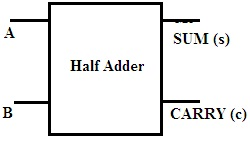
\includegraphics[width=0.5\linewidth]{./image/Half-Adder-blockblock.jpg}
	\caption{Bộ Half Adder}
	\label{f_block haft adder}
\end{figure}

Ta có bảng sự thật của mạch:

\begin{table}[H]
	\centering
	\begin{tabular}{|c|c|c|c|}
		\hline
		\multicolumn{2}{|c|}{Input} & \multicolumn{2}{c|}{Output} \\
		\hline
		A & B & SUM(S) & CARRY(C) \\
		\hline
		0 & 0 & 0 & 0 \\
		\hline
		0 & 1 & 1 & 0 \\
		\hline
		1 & 0 & 1 & 0 \\
		\hline
		1 & 1 & 0 & 1 \\
		\hline
	\end{tabular}
	\caption{Bảng sự thật của bộ Half Adder}
	\label{t_true table}
\end{table}

Thực hiện bộ Half Adder:
\begin{itemize}[label = -]
	\item Bộ Half Adder thực hiện bảng cổng XOR và cổng AND:
	\begin{figure}[H]
		\centering
		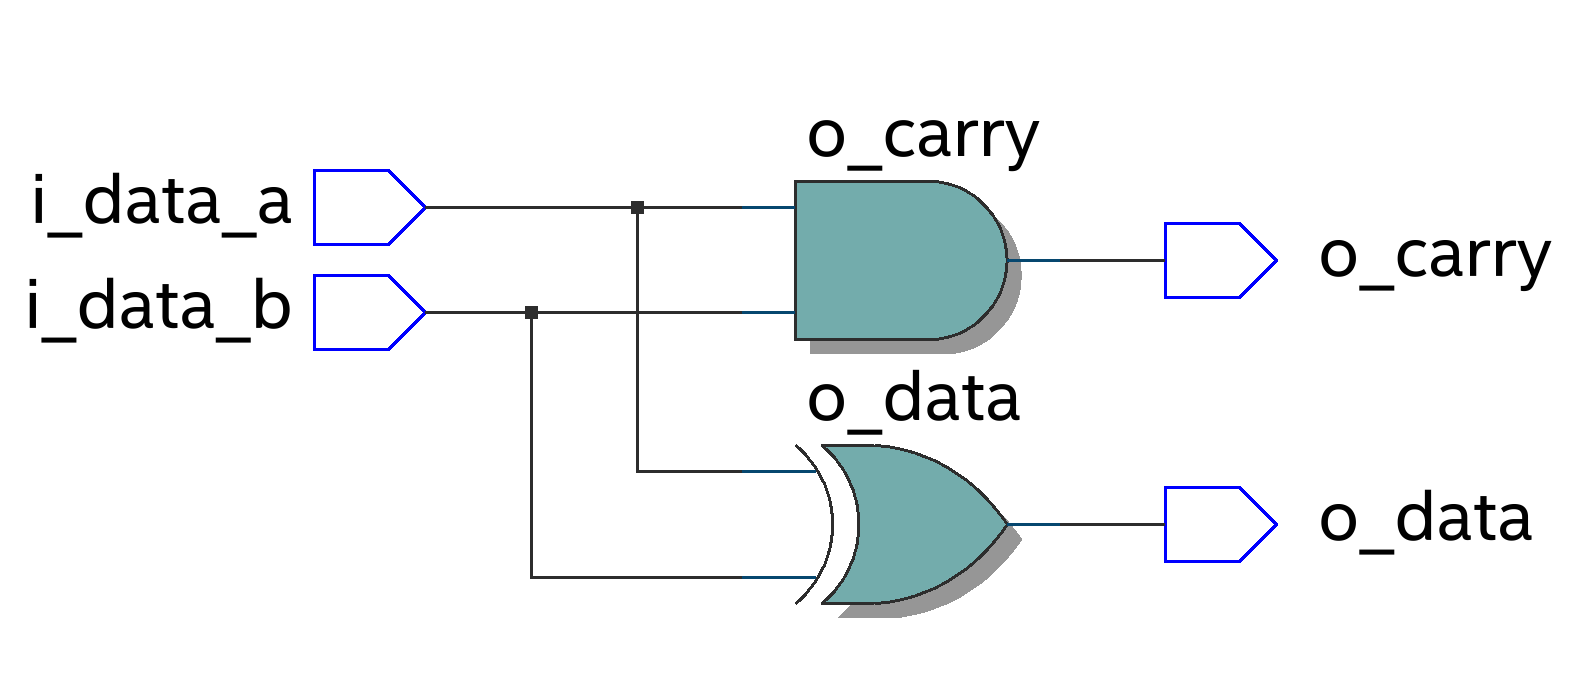
\includegraphics[width = 0.5\linewidth]{./image/half_adder_xor_and.png}
		\caption{Bộ Half Adder thực hiện bẳng cổng XOR và cổng AND}
		\label{f_half adder with xor and and}
	\end{figure}
	
	\lstinputlisting[style = SystemVerilog, caption = {Bộ Half Adder thực hiện bằng cổng XOR và cổng AND}]{./code/half_adder/half_adder_with_xor_and.sv}
	\item Bộ Half Adder thực hiện bẳng cổng NOR:
	\begin{figure}[H]
		\centering
		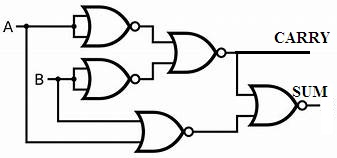
\includegraphics[width = .5\linewidth]{./image/Half-Adder-using-NOR-gates.jpg}
		\caption{Bộ Half Adder thực hiện bằng cổng NOR}
		\label{f_half adder with nor}
	\end{figure}
	
	\lstinputlisting[style=SystemVerilog, caption={Bộ Half Adder thực hiện bằng cổng NOR}]{./code/half_adder/half_adder_with_nor.sv}
	\item Bộ Half Adder thực hiện bằng cổng NAND:
	\begin{figure}[H]
		\centering
		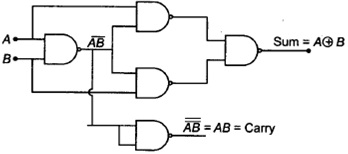
\includegraphics[width = 0.5\linewidth]{./image/Half-Adder-NAND-gates.jpg}
		\caption{Bộ Half Adder thực hiện bằng cổng NAND}
		\label{f_half adder with nand}
		
		\lstinputlisting[style=SystemVerilog, caption={Bộ Half Adder thực hiện bằng cổng NAND}]{./code/half_adder/half_adder_with_nand.sv}
	\end{figure}
\end{itemize}

Sử dụng test case sau đây để tiến hành kiểm tra lại hệ thống trên:
\begin{lstlisting}[style = C, caption={Test bench của bộ Half Adder}]
	int main(int argc, char **argv) {
		Verilated::commandArgs(argc, argv);
		
		VName_module* uut = new VName_module;
		
		// Test case
		printf("A B | Sum Carry\n");
		printf("-------------------\n");
		
		// case 1: A = 0, B = 0
		uut->i_data_a = 0; 
		uut->i_data_b = 0;
		uut->eval();
		printf("%d %d |  %d    %d\n", uut->i_data_a, uut->i_data_b, uut->o_data, uut->o_carry);
		
		// case 2: A = 0, B = 1
		uut->i_data_a = 0; 
		uut->i_data_b = 1;
		uut->eval();
		printf("%d %d |  %d    %d\n", uut->i_data_a, uut->i_data_b, uut->o_data, uut->o_carry);
		
		// case 3: A = 1, B = 0
		uut->i_data_a = 1; 
		uut->i_data_b = 0;
		uut->eval();
		printf("%d %d |  %d    %d\n", uut->i_data_a, uut->i_data_b, uut->o_data, uut->o_carry);
		
		// case 4: A = 1, B = 1
		uut->i_data_a = 1; 
		uut->i_data_b = 1;
		uut->eval();
		printf("%d %d |  %d    %d\n", uut->i_data_a, uut->i_data_b, uut->o_data, uut->o_carry);
		
		// deleted object
		delete uut;
		return 0;
	}
\end{lstlisting}

Kết quả:


	\begin{lstlisting}[style = C, caption={Sử dụng cổng XOR và cổng AND}]
		$ ./obj_dir/Vhalf_adder_with_xor_and 
		A B | Sum Carry
		-------------------
		0 0 |  0    0
		0 1 |  1    0
		1 0 |  1    0
		1 1 |  0    1
	\end{lstlisting}
	
	\begin{lstlisting}[style=C, caption={Sử dụng cổng NOR}]
		$ ./obj_dir/Vhalf_adder_with_nor 
		A B | Sum Carry
		-------------------
		0 0 |  0    0
		0 1 |  1    0
		1 0 |  1    0
		1 1 |  0    1
	\end{lstlisting}
	
	\begin{lstlisting}[style = C, caption={Sử dụng cổng NAND}]
		$ ./obj_dir/Vhalf_adder_with_nand
		A B | Sum Carry
		-------------------
		0 0 |  0    0
		0 1 |  1    0
		1 0 |  1    0
		1 1 |  0    1
	\end{lstlisting}
	
	\section{Full Adder}
		Bộ Full Adder là một mạch logic số dùng để cộng 3-bit nhị phân, thường đầu vào được biểu diễn dưới dạng $A$, $B$, và $C_{in}$ (bit nhớ), đầu ra được biểu diễn dưới dạng $\text{SUM}(s)$ và $C_{out}$ (bit nhớ). Với $\text{SUM}(s) = A \oplus B \oplus C_{in}$ và $C_{out} = (A \& B) \| (C_{in} \& (A \oplus B))$.

\begin{figure}[H]
	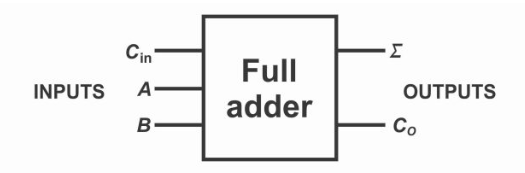
\includegraphics[width = 0.5\linewidth]{./image/full adder block.png}
	\centering
	\caption{Bộ Full Adder}
	\label{f_full adder block}	
\end{figure}

Bảng sự thật:

\begin{table}[H]
	\centering
	\begin{tabular}{|c|c|c|c|c|}
		\hline
		\multicolumn{3}{|c|}{Input} & \multicolumn{2}{c|}{Output}\\
		\hline
		$A$ & $B$ & $C_{in}$ & $\text{SUM}(s)$ & $C_{out}$\\
		\hline
		0 & 0 & 0 & 0 & 0\\
		\hline
		0 & 0 & 1 & 1 & 0\\
		\hline
		0 & 1 & 0 & 1 & 0\\
		\hline
		0 & 1 & 1 & 0 & 1\\
		\hline
		1 & 0 & 0 & 1 & 0\\
		\hline
		1 & 0 & 1 & 0 & 1\\
		\hline
		1 & 1 & 0 & 0 & 1\\
		\hline
		1 & 1 & 1 & 1 & 1\\
		\hline
	\end{tabular}
	\caption{Bảng sự thật của bộ Full Adder}
	\label{t_true table}
\end{table}

Thực hiện bộ Full Adder:

\begin{itemize}[label = -]
	\item Bộ Full Adder thực hiện bằng cổng logic:\\
		\begin{figure}[H]
			\centering
			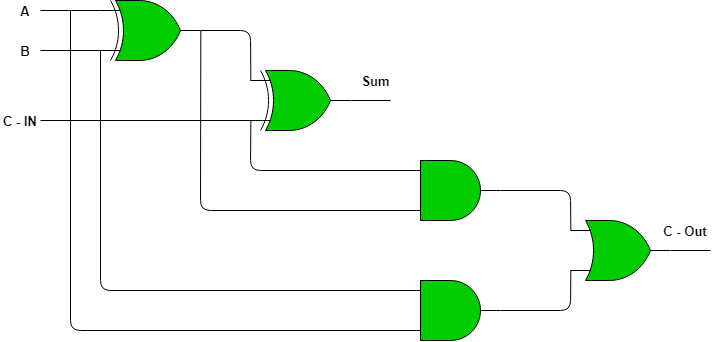
\includegraphics[width = .5\linewidth]{./image/full_adder_circuitcircuit.png}
			\caption{Bộ Full Adder thực hiện bằng cổng logic}
			\label{f_full adder circuit}
		\end{figure}
		
		\lstinputlisting[style=SystemVerilog, caption={Bộ Full Adder thực hiện bằng cổng logic}]{./code/full_adder/full_adder_circuit.sv}logic
	\item Bộ Full Adder thực hiện bằng bộ Half Adder:\\
		\begin{figure}[H]
			\centering
			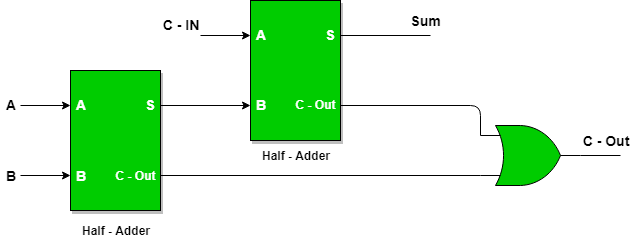
\includegraphics[width = 0.5\linewidth]{./image/full_adder_with_half_adder.png}
			\caption{Bộ Full Adder thực hiện bằng các bộ Half Adder}
			\label{f_full adder with half adder}
		\end{figure}
		
		\lstinputlisting[style=C, caption={Bộ Full Adder thực hiện bằng bộ Half Adder}]{./code/full_adder/full_adder_with_half_adder.sv}
\end{itemize}

Sử dụng các test case sau để kiểm tra hệ thống:

\begin{lstlisting}[style=C, caption={Test bench của bộ Full Adder}]
	#include <iostream>
	#include <verilated.h>
	#include "VName_moduel.h" // Verilator-generated header file
	
	int main(int argc, char **argv) {
		// Initialize Verilator
		Verilated::commandArgs(argc, argv);
		
		// Create an instance of the module
		VName_moduel* dut = new VName_moduel;
		
		// Input test vectors
		int test_cases[8][3] = {
			{0, 0, 0}, // {i_data_a, i_data_b, i_carry}
			{0, 0, 1},
			{0, 1, 0},
			{0, 1, 1},
			{1, 0, 0},
			{1, 0, 1},
			{1, 1, 0},
			{1, 1, 1},
		};
		
		// Print table header
		std::cout << "A B Cin | Sum Cou" << std::endl;
		std::cout << "--------|--------" << std::endl;
		
		// Run test cases
		for (int i = 0; i < 8; ++i) {
			// Apply inputs
			dut->i_data_a = test_cases[i][0];
			dut->i_data_b = test_cases[i][1];
			dut->i_carry  = test_cases[i][2];
			
			// Evaluate the circuit
			dut->eval();
			
			// Display inputs and outputs
			std::cout << test_cases[i][0] << " "
			<< test_cases[i][1] << "   "
			<< test_cases[i][2] << "  |   "
			<< (int)dut->o_data << "   "
			<< (int)dut->o_carry << std::endl;
		}
		
		// Cleanup
		delete dut;
		
		return 0;
	}
\end{lstlisting}

Kết quả:

\begin{lstlisting}[style=C, caption={Kết quả của test bench của bộ Full Adder sử dụng cổng logic}]
	$ ./obj_dir/Vfull_adder_circuit 
	A B Cin | Sum Cou
	--------|--------
	0 0   0  |   0   0
	0 0   1  |   1   0
	0 1   0  |   1   0
	0 1   1  |   0   1
	1 0   0  |   1   0
	1 0   1  |   0   1
	1 1   0  |   0   1
	1 1   1  |   1   1
\end{lstlisting}


\begin{lstlisting}[style=C, caption={Kết quả của test bench của bộ Full Adder sử dụng bộ Half Adder}]
	$ ./obj_dir/Vfull_adder_with_half_adder 
	A B Cin | Sum Cou
	--------|--------
	0 0   0  |   0   0
	0 0   1  |   1   0
	0 1   0  |   1   0
	0 1   1  |   0   1
	1 0   0  |   1   0
	1 0   1  |   0   1
	1 1   0  |   0   1
	1 1   1  |   1   1
\end{lstlisting}
	
	\section{Ripple Carry Adder (RCA)}
		Ripple Carry Adder (RCA) là một bộ cộng số học trong thiết kế mạch số, được sử dụng để cộng hai số nhị phân. RCA hoạt động dựa trên nguyên tắc tính toán carry (bit nhớ) theo kiểu tuần tự (ripple), tức là carry của mỗi bit phụ thuộc vào carry từ bit trước đó. Bộ Ripple Carry Adder được cấu tạo từ nhiều bộ Full Adder (FA) kết nối tuần tự với nhau.

\begin{figure}[H]
	\centering
	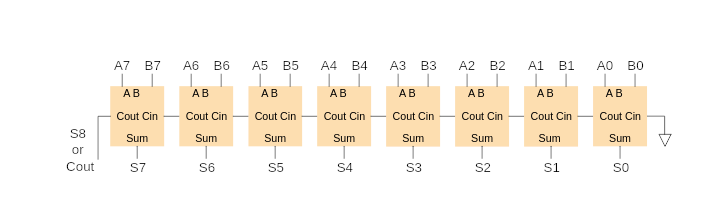
\includegraphics[width = 0.7\linewidth]{./image/ripple_carry_structure.png}
	\caption{Cấu trúc bộ Ripple Carry Adder}
	\label{f_diagam ripple carry adder}
\end{figure}

Trong đó:\\
\begin{itemize}[label = -]
	\item Tổng ($S_{i}$): $S_{i} = A_{i} \oplus B_{i} \oplus C_{i}$.
	\item Carry ($C_{i+1}$): $C_{i+1} = (A_{i} \& B_{i}) + (C_{i} \& (A_{i} \oplus B_{i}))$ 
\end{itemize}

\begin{itemize}[label = -]
	\item Ưu điểm: 
		\begin{itemize}[label = +]
			\item Thiết kế đơn giản, mỗi bit được xử lý bằng bộ Full Adder được kết nối theo chuỗi.
			\item Tiết kiệm tài nguyên phần cứng, phù hợp cho các hoạt động không yêu cầu quá cao về hiệu suất.
			\item Dễ dàng mở rộng mà không cần thay đổi quá nhiều vào logic của mạch.
			\item Tiết kiệm chi phí vì sử dụng ít cổng logic.
		\end{itemize}
	\item Nhược điểm:
		\begin{itemize}[label = +]
			\item Độ trễ cao do phải xử lý tuần tự, độ trễ tăng tuyến tính theo n-bit, với độ trễ được tính bằng \[ T_{delay} = n \times T_{unit} \] với, $T_{unit}$ là độ trễ của từng khối trong RCA.
			\item Hiệu suất thấp đối với số lượng bit lớn.
			\item Không tối ưu khi hệ thống yêu cầu thời gian thực vì có độ trễ lớn.
			\item Giới hạn hoạt động do tính tuần tự nên hệ thống RCA bị giới hạn tần số hoạt động, không đáp ứng ở hệ thống hoạt động ở tần số cao.
		\end{itemize}
\end{itemize}

\begin{lstlisting}[style = SystemVerilog, caption={RCA}]
	module rca (
	input logic [31:0]  i_data_a,  // Operand A
	input logic [31:0]  i_data_b,  // Operand B
	output logic [31:0] o_data     // Sum output
	);
	
	logic [31:0] carry; // Carry signals
	
	// Instance of the first full adder (LSB)
	full_adder FA0 (
	.i_data_a(i_data_a[0]),
	.i_data_b(i_data_b[0]),
	.i_carry(1'b0),          // Initial carry-in is 0
	.o_data(o_data[0]),
	.o_carry(carry[0])
	);
	
	// Instances of remaining 31 full adders
	full_adder FA1  (.i_data_a(i_data_a[1]),  .i_data_b(i_data_b[1]),  .i_carry(carry[0]), .o_data(o_data[1]),  .o_carry(carry[1]));
	full_adder FA2  (.i_data_a(i_data_a[2]),  .i_data_b(i_data_b[2]),  .i_carry(carry[1]), .o_data(o_data[2]),  .o_carry(carry[2]));
	full_adder FA3  (.i_data_a(i_data_a[3]),  .i_data_b(i_data_b[3]),  .i_carry(carry[2]), .o_data(o_data[3]),  .o_carry(carry[3]));
	full_adder FA4  (.i_data_a(i_data_a[4]),  .i_data_b(i_data_b[4]),  .i_carry(carry[3]), .o_data(o_data[4]),  .o_carry(carry[4]));
	full_adder FA5  (.i_data_a(i_data_a[5]),  .i_data_b(i_data_b[5]),  .i_carry(carry[4]), .o_data(o_data[5]),  .o_carry(carry[5]));
	full_adder FA6  (.i_data_a(i_data_a[6]),  .i_data_b(i_data_b[6]),  .i_carry(carry[5]), .o_data(o_data[6]),  .o_carry(carry[6]));
	full_adder FA7  (.i_data_a(i_data_a[7]),  .i_data_b(i_data_b[7]),  .i_carry(carry[6]), .o_data(o_data[7]),  .o_carry(carry[7]));
	full_adder FA8  (.i_data_a(i_data_a[8]),  .i_data_b(i_data_b[8]),  .i_carry(carry[7]), .o_data(o_data[8]),  .o_carry(carry[8]));
	full_adder FA9  (.i_data_a(i_data_a[9]),  .i_data_b(i_data_b[9]),  .i_carry(carry[8]), .o_data(o_data[9]),  .o_carry(carry[9]));
	full_adder FA10 (.i_data_a(i_data_a[10]), .i_data_b(i_data_b[10]), .i_carry(carry[9]), .o_data(o_data[10]), .o_carry(carry[10]));
	full_adder FA11 (.i_data_a(i_data_a[11]), .i_data_b(i_data_b[11]), .i_carry(carry[10]), .o_data(o_data[11]), .o_carry(carry[11]));
	full_adder FA12 (.i_data_a(i_data_a[12]), .i_data_b(i_data_b[12]), .i_carry(carry[11]), .o_data(o_data[12]), .o_carry(carry[12]));
	full_adder FA13 (.i_data_a(i_data_a[13]), .i_data_b(i_data_b[13]), .i_carry(carry[12]), .o_data(o_data[13]), .o_carry(carry[13]));
	full_adder FA14 (.i_data_a(i_data_a[14]), .i_data_b(i_data_b[14]), .i_carry(carry[13]), .o_data(o_data[14]), .o_carry(carry[14]));
	full_adder FA15 (.i_data_a(i_data_a[15]), .i_data_b(i_data_b[15]), .i_carry(carry[14]), .o_data(o_data[15]), .o_carry(carry[15]));
	full_adder FA16 (.i_data_a(i_data_a[16]), .i_data_b(i_data_b[16]), .i_carry(carry[15]), .o_data(o_data[16]), .o_carry(carry[16]));
	full_adder FA17 (.i_data_a(i_data_a[17]), .i_data_b(i_data_b[17]), .i_carry(carry[16]), .o_data(o_data[17]), .o_carry(carry[17]));
	full_adder FA18 (.i_data_a(i_data_a[18]), .i_data_b(i_data_b[18]), .i_carry(carry[17]), .o_data(o_data[18]), .o_carry(carry[18]));
	full_adder FA19 (.i_data_a(i_data_a[19]), .i_data_b(i_data_b[19]), .i_carry(carry[18]), .o_data(o_data[19]), .o_carry(carry[19]));
	full_adder FA20 (.i_data_a(i_data_a[20]), .i_data_b(i_data_b[20]), .i_carry(carry[19]), .o_data(o_data[20]), .o_carry(carry[20]));
	full_adder FA21 (.i_data_a(i_data_a[21]), .i_data_b(i_data_b[21]), .i_carry(carry[20]), .o_data(o_data[21]), .o_carry(carry[21]));
	full_adder FA22 (.i_data_a(i_data_a[22]), .i_data_b(i_data_b[22]), .i_carry(carry[21]), .o_data(o_data[22]), .o_carry(carry[22]));
	full_adder FA23 (.i_data_a(i_data_a[23]), .i_data_b(i_data_b[23]), .i_carry(carry[22]), .o_data(o_data[23]), .o_carry(carry[23]));
	full_adder FA24 (.i_data_a(i_data_a[24]), .i_data_b(i_data_b[24]), .i_carry(carry[23]), .o_data(o_data[24]), .o_carry(carry[24]));
	full_adder FA25 (.i_data_a(i_data_a[25]), .i_data_b(i_data_b[25]), .i_carry(carry[24]), .o_data(o_data[25]), .o_carry(carry[25]));
	full_adder FA26 (.i_data_a(i_data_a[26]), .i_data_b(i_data_b[26]), .i_carry(carry[25]), .o_data(o_data[26]), .o_carry(carry[26]));
	full_adder FA27 (.i_data_a(i_data_a[27]), .i_data_b(i_data_b[27]), .i_carry(carry[26]), .o_data(o_data[27]), .o_carry(carry[27]));
	full_adder FA28 (.i_data_a(i_data_a[28]), .i_data_b(i_data_b[28]), .i_carry(carry[27]), .o_data(o_data[28]), .o_carry(carry[28]));
	full_adder FA29 (.i_data_a(i_data_a[29]), .i_data_b(i_data_b[29]), .i_carry(carry[28]), .o_data(o_data[29]), .o_carry(carry[29]));
	full_adder FA30 (.i_data_a(i_data_a[30]), .i_data_b(i_data_b[30]), .i_carry(carry[29]), .o_data(o_data[30]), .o_carry(carry[30]));
	full_adder FA31 (.i_data_a(i_data_a[31]), .i_data_b(i_data_b[31]), .i_carry(carry[30]), .o_data(o_data[31]), .o_carry()); // Final carry ignored
	
	endmodule
	
	module full_adder(
	input logic     i_data_a,
	input logic     i_data_b,
	input logic     i_carry,
	
	output logic    o_data,
	output logic    o_carry
	);
	
	wire xor1;
	
	assign xor1 = i_data_a ^ i_data_b;
	assign o_data = xor1 ^ i_carry;
	assign o_carry = (i_data_a & i_data_b) | (i_carry & xor1);
	
	endmodule
\end{lstlisting}

\begin{lstlisting}[style = C, caption={Kết quả của test}]
	$ ./obj_dir/Vrca
	=== Test bench for Ripple Carry Adder (RCA) ===
	[PASS] Test case 1: A = 149, B = 186, Expected = 335, Actual = 335
	[PASS] Test case 2: A = 143, B = 254, Expected = 397, Actual = 397
	[PASS] Test case 3: A = 4, B = 0, Expected = 4, Actual = 4
	...
	[PASS] Test case 97: A = 165, B = 214, Expected = 379, Actual = 379
	[PASS] Test case 98: A = 120, B = 128, Expected = 248, Actual = 248
	[PASS] Test case 99: A = 116, B = 42, Expected = 158, Actual = 158
	[PASS] Test case 100: A = 36, B = 2, Expected = 38, Actual = 38
	
	=== Test Summary ===
	Total Test Cases: 100
	PASS: 100
	FAIL: 0
\end{lstlisting}

	
	\section{Carry Look-Ahead Adder (CLA)}
		Carry Look-Ahead Adder (CLA) là một loại bộ cộng số học trong kỹ thuật số, được thiết kế để thực hiện phép cộng hai số nhị phân nhanh hơn so với bộ cộng thông thường (như Ripple Carry Adder - RCA). CLA đạt được tốc độ cao bằng cách tính toán các tín hiệu carry đồng thời (song song) thay vì tuần tự, nhờ vào các tín hiệu Generate (G) và Propagate (P). 

\begin{figure}[H]
	\centering
	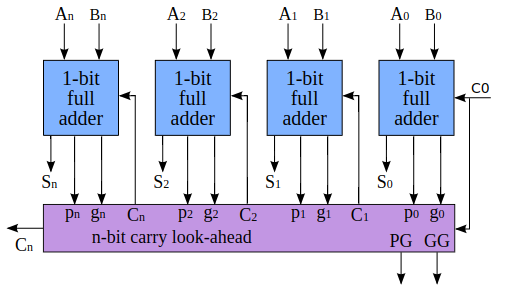
\includegraphics[width=0.5\linewidth]{./image/carry_look_ahead_structure.png}
	\caption{Cấu trúc của bộ Carry Look-Ahead}
	\label{f_carry look ahead structure}
\end{figure}

Trong đó,

\begin{itemize}[label = -]
	\item Generate $(G_{i})$: $G_{i} = A_{i} \cdot B_{i} $i.
	\item Propagate $(P_{i})$: $P_{i} = A_{i} + B_{i}$.
	\item Tổng $(S_{i})$: $S_{i} = G_{i} \cdot P_{i}$.
	\item Carry $(C_{i+1})$: $C_{i + 1} = G_{i} + P_{i}\cdot C_{i}$.
\end{itemize}

\begin{itemize}[label = -]
	\item Ưu điểm: 
	\begin{itemize}[label = +]
		\item Tốc độ xử lý cao do tín hiệu carry được xử lý song song.
		\item Giảm độ trễ với độ trễ tăng theo $O(\log_{2}(n))$, thay vì $O(n)$ như RCA.
	\end{itemize}
	\item Nhược điểm:
	\begin{itemize}[label = +]
		\item Phức tạp về thiết kế do yêu cầu xử dụng nhiều cổng logic để tính toán carry đồng thời, làm tăng độ phức tạp của hệ thống.
		\item Tốn tài nguyên phần cứng do số lượng cổng logic tăng nhanh khi số bit tăng, làm tăng chi phí phần cứng.
		\item Khó mở rộng do khi số bit lớn thì yêu cầu cần thiết kế phức tạp hơn, và việc tính toán carry đòi hỏi nhiều tài nguyên.
	\end{itemize}
\end{itemize}

\begin{lstlisting}[style = SystemVerilog, caption={CLA}]
	module cla (
	input  logic [31:0] i_data_a,   // Operand A (32-bit input)
	input  logic [31:0] i_data_b,   // Operand B (32-bit input)
	output logic [31:0] o_data,     // Sum output (32-bit)
	output logic        o_carry     // Carry-out (1-bit output)
	);
	logic [31:0] G, P;              // Bitwise Generate (G) and Propagate (P) signals
	logic [32:0] C;                 // Carry signals for each bit (including carry-out)
	
	// Generate and Propagate logic
	// G[i] = i_data_a[i] & i_data_b[i]: A carry is generated when both bits are 1.
	// P[i] = i_data_a[i] | i_data_b[i]: A carry is propagated if at least one of the bits is 1.
	assign G = i_data_a & i_data_b; // Generate signals
	assign P = i_data_a | i_data_b; // Propagate signals
	
	// Carry logic
	// C[0] is initialized to 0 because there is no carry-in for the least significant bit.
	// C[i+1] = G[i] | (P[i] & C[i]): Carry for the next bit depends on the current bit's generate or propagate conditions.
	assign C[0] = 0; // Initial carry-in is 0
	generate
	genvar i;
	for (i = 0; i < 32; i++) begin : carry_logic_block
	// Compute carry-out for each bit position
	assign C[i+1] = G[i] | (P[i] & C[i]);
	end
	endgenerate
	
	// Sum logic
	// o_data[i] = i_data_a[i] ^ i_data_b[i] ^ C[i]: The sum is computed using the XOR of the two operands and the carry-in for each bit.
	assign o_data = i_data_a ^ i_data_b ^ C[31:0]; // Sum computation
	assign o_carry = C[32]; // The final carry-out from the most significant bit
	endmodule
\end{lstlisting}

\begin{lstlisting}[style=C, caption={Kết quả test}]
	$ ./obj_dir/Vcla 
	=== Test bench for Ripple Carry Adder (RCA) ===
	[PASS] Test case 1: A = 234, B = 25, Expected = 259, Actual = 259
	[PASS] Test case 2: A = 30, B = 255, Expected = 285, Actual = 285
	[PASS] Test case 3: A = 120, B = 28, Expected = 148, Actual = 148
	[PASS] Test case 4: A = 194, B = 123, Expected = 317, Actual = 317
	...
	[PASS] Test case 99: A = 85, B = 175, Expected = 260, Actual = 260
	[PASS] Test case 100: A = 101, B = 30, Expected = 131, Actual = 131
	
	=== Test Summary ===
	Total Test Cases: 100
	PASS: 100
	FAIL: 0
\end{lstlisting}
	
	\section{Kogge-Stone Adder (KSA)}
		Kogge-Stone Adder (KSA) là một bộ cộng song song hiệu suất cao được thiết kế để tính toán tín hiệu carry một cách nhanh chóng bằng cách sử dụng cấu trúc prefix network. Đây là một trong những loại Parallel Prefix Adders được sử dụng phổ biến nhất trong các bộ xử lý hiện đại, nhờ khả năng giảm độ trễ tính toán của tín hiệu carry xuống mức tối thiểu.

\begin{itemize}[label = -]
	\item Ưu điểm: 
	\begin{itemize}[label = +]
		\item Tốc độ xử lý nhanh, độ trễ tính toán carry giảm xuống $O(\log_{2}(n))$, rất nhanh đối với số bit lớn.
		\item Khả năng tính toán trong từng cấp có thể thực hiện đồng thời, cải thiện hiệu suất.
		\item Thích hợp cho tính toán số bit lớn như 32-bit, 64-bit, 128-bit hoặc lớn. 
	\end{itemize}
	\item Nhược điểm:
	\begin{itemize}[label = +]
		\item Tài nguyên phần cứng lớn do cần nhiều cổng logic rất lớn, đặc biết đối với các số bit lớn.
		\item Độ phức tạp thiết kế cao do cấu trúc mạng prèĩ đòi hỏi thiết kế phức tạp, khó tối ưu hóa cho chi phí.
		\item Tiêu thụ năng lượng cao do sử dụng lượng lớn cổng logic và phép tính đồng thời.
	\end{itemize}
\end{itemize}
		
	\section{Index}
		\begin{lstlisting}[style = C, caption={Test case cho Bộ cộng}]
	#include <iostream>
	#include <verilated.h>
	#include <cstdlib>  // For rand() and srand()
	#include <ctime>    // For time()
	
	#include "Vrca.h"
	
	int main(int argc, char** argv) {
		// Initialize Verilator
		Verilated::commandArgs(argc, argv);
		std::cout << "=== Test bench for Ripple Carry Adder (RCA) ===" << std::endl;
		
		// Create an instance of the RCA module
		Vrca* dut = new Vrca;
		
		// Initialize random seed
		srand(static_cast<unsigned>(time(0)));
		
		// Variables to track results
		int pass_count = 0;
		int fail_count = 0;
		
		// Run 100 test cases
		for (int i = 0; i < 100; ++i) {
			// Generate random inputs
			int a = rand() % 256;  // Random 8-bit value (0 to 255)
			int b = rand() % 256;  // Random 8-bit value (0 to 255)
			int expected_sum = a + b;  // Expected result
			
			// Apply inputs to the DUT
			dut->i_data_a = a;
			dut->i_data_b = b;
			
			// Evaluate the DUT
			dut->eval();
			
			// Capture output
			int actual_sum = dut->o_data;
			
			// Check for correctness
			if (actual_sum == expected_sum) {
				++pass_count;
				std::cout << "[PASS] Test case " << i + 1 << ": A = " << a << ", B = " << b
				<< ", Expected = " << expected_sum << ", Actual = " << actual_sum << std::endl;
			} else {
				++fail_count;
				std::cout << "[FAIL] Test case " << i + 1 << ": A = " << a << ", B = " << b
				<< ", Expected = " << expected_sum << ", Actual = " << actual_sum << std::endl;
			}
		}
		
		// Display summary
		std::cout << "\n=== Test Summary ===" << std::endl;
		std::cout << "Total Test Cases: 100" << std::endl;
		std::cout << "PASS: " << pass_count << std::endl;
		std::cout << "FAIL: " << fail_count << std::endl;
		
		// Cleanup
		delete dut;
		return 0;
	}
\end{lstlisting}
\end{document}